%%%%%%%%%%%%%%%%%%%%%%%%%%%%%%%%%%%%%%%%%
% baposter Landscape Poster
% LaTeX Template
% Version 1.0 (11/06/13)
%
% baposter Class Created by:
% Brian Amberg (baposter@brian-amberg.de)
%
% This template has been downloaded from:
% http://www.LaTeXTemplates.com
%
% License:
% CC BY-NC-SA 3.0 (http://creativecommons.org/licenses/by-nc-sa/3.0/)
%
%%%%%%%%%%%%%%%%%%%%%%%%%%%%%%%%%%%%%%%%%

%----------------------------------------------------------------------------------------
%	PACKAGES AND OTHER DOCUMENT CONFIGURATIONS
%----------------------------------------------------------------------------------------

\documentclass[portrait,a0paper,fontscale=0.31]{baposter} % Adjust the font scale/size here

\usepackage[absolute,overlay]{textpos} % For absolute positioning
\usepackage{graphicx} % For graphics
\usepackage{multirow} % For merging cells across several rows
\usepackage{array}    % For customizing the column format
\usepackage{enumitem}

\usepackage{graphicx} % Required for including images
\graphicspath{{figures/}} % Directory in which figures are stored

\usepackage{amsmath} % For typesetting math
\usepackage{amssymb} % Adds new symbols to be used in math mode

\usepackage{breqn}  % Used for breaking equations on multiple lines


\usepackage{booktabs} % Top and bottom rules for tables
\usepackage{enumitem} % Used to reduce itemize/enumerate spacing
\usepackage{palatino} % Use the Palatino font
\usepackage[font=small,labelfont=bf]{caption} % Required for specifying captions to tables and figures

\usepackage{multicol} % Required for multiple columns
\setlength{\columnsep}{1.5em} % Slightly increase the space between columns
\setlength{\columnseprule}{0mm} % No horizontal rule between columns

\usepackage{tikz} % Required for flow chart
\usetikzlibrary{shapes,arrows} % Tikz libraries required for the flow chart in the template

\usepackage{graphicx} % Required for including images and floating tables/figures
\usepackage{amsmath} % For advanced math formatting
\usepackage{amssymb} % For additional math symbols
\usepackage{float} % For the [H] specifier, which forces the table to be placed exactly where it appears in the code
\usepackage{booktabs} % For enhanced table formatting


%%%%%%%%%%
\usepackage{cite}
\usepackage{amsmath,amssymb,amsfonts}
\usepackage{graphicx}
\usepackage{textcomp}
\usepackage{float}
\usepackage{xcolor}
\usepackage[english]{babel}
% \usepackage{hyperref}
%%%%%%%%%%

\newcommand{\compresslist}{ % Define a command to reduce spacing within itemize/enumerate environments, this is used right after \begin{itemize} or \begin{enumerate}
\setlength{\itemsep}{1pt}
\setlength{\parskip}{0pt}
\setlength{\parsep}{0pt}
}

\definecolor{lightblue}{rgb}{0.145,0.6666,1} % Defines the color used for content box headers

\definecolor{udesa}{RGB}{0, 18, 187}

\begin{document}

\begin{poster}
{
headerborder=closed, % Adds a border around the header of content boxes
colspacing=1em, % Column spacing
bgColorOne=white, % Background color for the gradient on the left side of the poster
bgColorTwo=white, % Background color for the gradient on the right side of the poster
borderColor=udesa, % Border color
headerColorOne=udesa, % Background color for the header in the content boxes (left side)
headerColorTwo=udesa, % Background color for the header in the content boxes (right side)
headerFontColor=white, % Text color for the header text in the content boxes
boxColorOne=white, % Background color of the content boxes
textborder=rounded, % Format of the border around content boxes, can be: none, bars, coils, triangles, rectangle, rounded, roundedsmall, roundedright or faded
eyecatcher=true, % Set to false for ignoring the left logo in the title and move the title left
headerheight=0.1\textheight, % Height of the header
headershape=roundedright, % Specify the rounded corner in the content box headers, can be: rectangle, small-rounded, roundedright, roundedleft or rounded
headerfont=\Large\bf, % Large, bold and sans serif font in the headers of content boxes
%textfont={\setlength{\parindent}{1.5em}}, % Uncomment for paragraph indentation
linewidth=2pt % Width of the border lines around content boxes
}
%----------------------------------------------------------------------------------------
%	Title
%----------------------------------------------------------------------------------------
%
{
\includegraphics[height=7em]{figures/UDESA.png}} % First university/lab logo on the left
{\Large{I302 - Machine Learning and Deep Learning - Universidad de San Andrés - 2025}\vspace{0.35cm}\\\Huge\bf{ECG Anomaly Detection using Latent Representations and Reconstruction Error of a VAE}\vspace{0.35cm}} % Poster title
{Ana Paula Tissera (atissera@udesa.edu.ar), Naomi Couriel (ncouriel@udesa.edu.ar)} % Author names and institution

% batch{
\includegraphics[height=7em]{figures/UDESA.png}} % Second university/lab logo on the right


\headerbox{Introduction}{name=resumen,column=0,row=0}{

\hspace*{0.5em} Manual analysis of ECG (electrocardiographic) signals is a costly, slow process that is highly dependent on specialists, which hinders its scalability in high-demand clinical settings. Given the growing need for diagnoses, we seek to develop automatic tools capable of reliably detecting anomalies.
}

\headerbox{Objectives}{name=objetivos,column=0,below= resumen}{

\begin{itemize}[left=0.45em, rightmargin=0.6em]
  \item Learn latent representations of normal ECG signals using a 1D VAE.
  \item Detect anomalies from the VAE reconstruction error.
  \item Classify anomalous signals using an XGBoost classifier over the latent vectors and the reconstruction score.
  \item Evaluate the pipeline's performance on the public PTB-XL and Chapman-Shaoxing databases.
\end{itemize}
}

%----------------------------------------------------------------------------------------
%	Data and FMM
%----------------------------------------------------------------------------------------

\headerbox{Data \& FMM}{name=details,column=0,below=objetivos}{

\textbf{Datasets used}
\begin{itemize}[left=0.45em, rightmargin=0.6em]
    \item \textit{PTB-XL ECG Dataset}: 21,837 12-lead records, 500 Hz.
    \item \textit{Chapman-Shaoxing ECG Dataset}: 10,646 multi-class arrhythmia records.
\end{itemize}

\textbf{Morphological features (FMM) and preprocessing}

\hspace*{0.7em} 21 coefficients were extracted that characterize the P, Q, R, S and T waves through the Frequency Modulated Möbius model, describing their amplitudes, phases, directionality and frequencies.

\vspace{-0.20cm}
\begin{figure}[H]
    \centering
    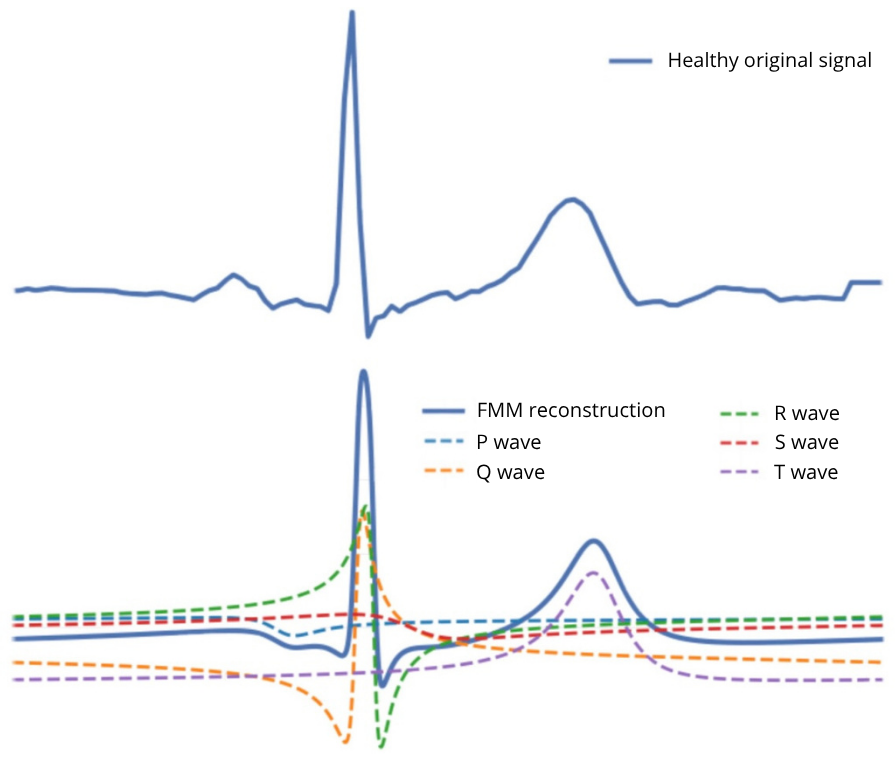
\includegraphics[width=0.9\textwidth]{ourfigures/señalesconFMM_conlabels.png}
    \caption{ECG signal and its reconstruction using the FMM model.}
\end{figure}

\vspace{-0.30cm}
\hspace*{0.7em} The ECG windows were resized to a fixed length of 2048 samples and each one was Z-score normalized using the statistics computed over the training set.

\vspace{0.20cm}


}




\headerbox{References}{name=ref,column=0,below=details}{

\renewcommand{\section}[2]{\vskip 0.05em} % Get rid of the default "References" section title

\vspace{0.3em}

\begin{thebibliography}{9}

\bibitem{verardo2023fmmhead}
Verardo, Boman, Bruchfeld, Chiesa, Koch, Maguire Jr., and Kostic.
\textit{FMM-Head: Enhancing Autoencoder-based ECG anomaly detection with prior knowledge}, 2023.
\vspace{0.25em}

\bibitem{jang2021unsupervised}
Jang, Kim, Lim, and Yoon.
\textit{Unsupervised feature learning for electrocardiogram data using the convolutional variational autoencoder}, 2021.

\end{thebibliography}
\vspace{0.22em}


\small

% keeps the bottom of column 0 level with the Results box
\vspace{0cm}

%\vspace{0.25cm}

%\nocite{*} % Insert publications even if they are not cited in the poster
%\small{ % Reduce the font size in this block
%\bibliographystyle{unsrt}
%\bibliography{suvs_poster} % Use sample.bib as the bibliography file

%\vspace{0.0875cm}

}





%----------------------------------------------------------------------------------------
%	Architecture
%----------------------------------------------------------------------------------------

\headerbox{Variational Autoencoder}{name=arquitectura,column=1}{
\hspace*{0.7em} The VAE compresses each ECG window together with its FMM coefficients into a latent space and then reconstructs it, so that the reconstruction error (ELBO) serves as an anomaly indicator.
\vspace{-0.051cm}
\begin{figure}[H]
    \centering
    
\includegraphics[width=0.9\textwidth]{ourfigures/vaearc.png}
    \caption{VAE architecture}
\end{figure}

\vspace{-5mm}

\begin{figure}[H]
    \centering
    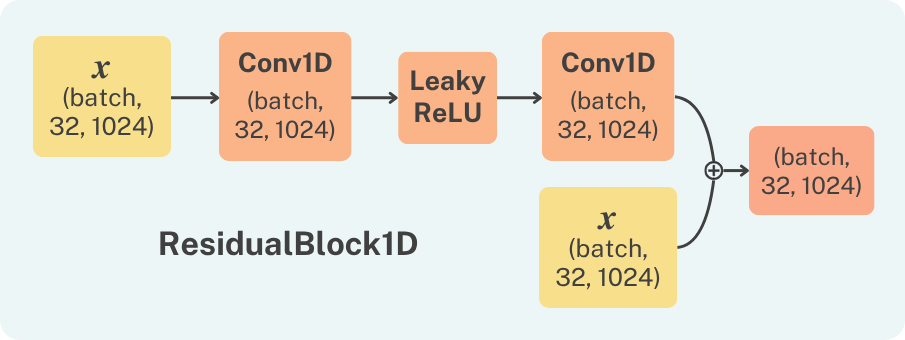
\includegraphics[width=0.78\textwidth]{ourfigures/resb1darc.png}
    \caption{1D Resize Block architecture}
\end{figure}
\vspace{-0.4cm}

\begin{enumerate}[left=0.45em, rightmargin=0.6em]
  \item \textbf{Encoder}: takes as input the ECG signal (2048 samples) and the FMM coefficient vector.
        It extracts features and projects them into two latent parameter vectors, \(\mu\) and \(\log\sigma^2\).
  \item \textbf{Reparameterization}: from \(\mu\) and \(\log\sigma^2\) we sample
        \vspace{-0.3cm}
        \[
          z = \mu + \sigma \odot \epsilon,\quad \epsilon \sim \mathcal{N}(0,I).
        \]
        \vspace{-0.8cm}
  \item \textbf{Decoder}: takes \(z\) and generates the reconstruction \(\hat{x}\) of the ECG window, trying to approximate the original signal.
\end{enumerate}

}

%----------------------------------------------------------------------------------------
%	Anomaly score
%----------------------------------------------------------------------------------------


\headerbox{Anomaly Score}{name=elbo,column=2}{

\hspace*{0.5em} The anomaly score is the ELBO, combining reconstruction error and latent regularization:
\vspace{-0.2cm}
\[
  \mathrm{ELBO} = -\underbrace{\mathrm{MSE}(\hat{x},x)}_{\text{reconstruction}}
                -\beta\, \underbrace{\mathrm{KL}\bigl(q(z\mid x)\;\Vert\;\mathcal{N}(0,I)\bigr)}_{\text{regularization}}.
\]

}


\headerbox{XGBoost}{name=xgboost,column=2, below=elbo}{

\hspace*{0.5em} For each beat we build $\mathbf{c} = [\boldsymbol{\mu}, e] \in \mathbb{R}^{65}$ from the latent mean $\boldsymbol{\mu}$ and the reconstruction error $e$. An XGBoost classifier maps it to the final prediction (\textit{Normal} vs. \textit{Anomalous}).
\vspace{-0.1cm}

\begin{figure}[H]
    \centering
    
\includegraphics[width=0.85\textwidth]{ourfigures/xgboost.png}
    \caption{XGBoost classifier}
\end{figure}




}



\headerbox{Conclusions \& Future Work}{name=conclu,column=2,below=xgboost}{
\vspace{0.30cm}
\begin{itemize}[left=0.45em, rightmargin=0.6em]
    \item The VAE + XGBoost pipeline recovers 74\% of the anomalous beats on unseen patients.
    \item FMM coefficients add useful morphological prior knowledge.
    \item Splitting by recording instead of by beat is essential: it lowers validation AUC from 0.91 to 0.85.
    \item In the future, attention mechanisms or synthetic data could be incorporated.

\vspace{0.30cm}

\end{itemize}

}




%----------------------------------------------------------------------------------------
%	Results
%----------------------------------------------------------------------------------------

\headerbox{Results}{name=resultados,column=1,span=2, below=arquitectura}{


%\vspace{0.5em}

\begin{center}
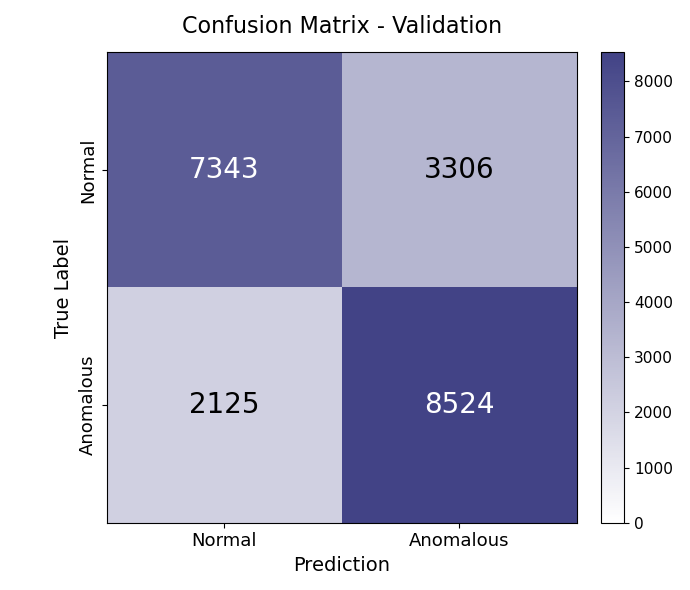
\includegraphics[width=0.3\textwidth]{ourfigures/matconfval2.png}
\hspace{2em}
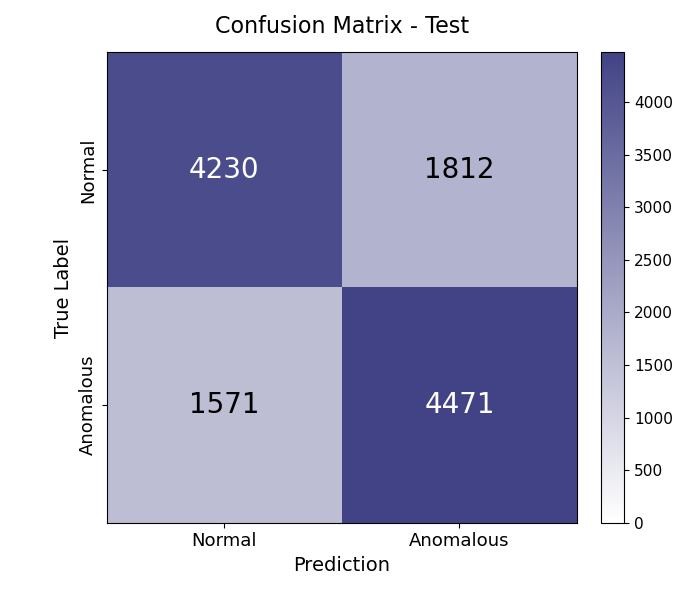
\includegraphics[width=0.3\textwidth]{ourfigures/matconftest2.png}

\vspace{0.3em}
\small
Confusion matrices: validation (left) and test (right)
\end{center}

\vspace{-0.25em}

All splits are grouped by recording, so no patient appears in more than one split. The threshold is picked on validation to keep recall above 0.80.
\vspace{-0.1cm}

\small
\begin{center}
\begin{tabular}{lcc}
\toprule
\textbf{Metric} & \textbf{Validation} & \textbf{Test} \\
\midrule
AUC-ROC   & 0.8503 & 0.8058 \\
Precision & 0.7399 & 0.7116 \\
Recall    & 0.8001 & 0.7400 \\
F1-score  & 0.7688 & 0.7255 \\
Accuracy  & 0.7594 & 0.7200 \\
\bottomrule
\end{tabular}
\end{center}


}







% \begin{textblock*}{7cm}(3cm, 34.5cm) % 5cm width, (3cm, 4cm) is the position on the page
%     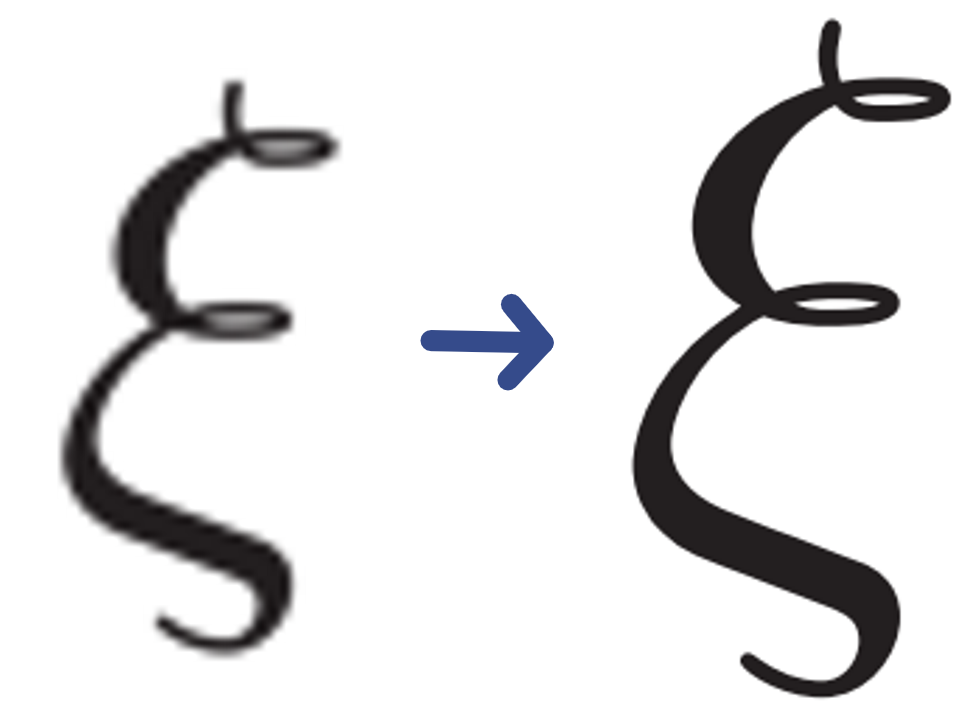
\includegraphics[width=1.5cm]{figures/xi.png} % Include the image at the specified position
% \end{textblock*}

%----------------------------------------------------------------------------------------
% Adjustments for the rest of the document
%----------------------------------------------------------------------------------------

% Remember to replace the images and references in the code as appropriate.

\end{poster}

\end{document}
